% Options for packages loaded elsewhere
\PassOptionsToPackage{unicode}{hyperref}
\PassOptionsToPackage{hyphens}{url}
\documentclass[
]{article}
\usepackage{xcolor}
\usepackage[margin=1in]{geometry}
\usepackage{amsmath,amssymb}
\setcounter{secnumdepth}{-\maxdimen} % remove section numbering
\usepackage{iftex}
\ifPDFTeX
  \usepackage[T1]{fontenc}
  \usepackage[utf8]{inputenc}
  \usepackage{textcomp} % provide euro and other symbols
\else % if luatex or xetex
  \usepackage{unicode-math} % this also loads fontspec
  \defaultfontfeatures{Scale=MatchLowercase}
  \defaultfontfeatures[\rmfamily]{Ligatures=TeX,Scale=1}
\fi
\usepackage{lmodern}
\ifPDFTeX\else
  % xetex/luatex font selection
\fi
% Use upquote if available, for straight quotes in verbatim environments
\IfFileExists{upquote.sty}{\usepackage{upquote}}{}
\IfFileExists{microtype.sty}{% use microtype if available
  \usepackage[]{microtype}
  \UseMicrotypeSet[protrusion]{basicmath} % disable protrusion for tt fonts
}{}
\makeatletter
\@ifundefined{KOMAClassName}{% if non-KOMA class
  \IfFileExists{parskip.sty}{%
    \usepackage{parskip}
  }{% else
    \setlength{\parindent}{0pt}
    \setlength{\parskip}{6pt plus 2pt minus 1pt}}
}{% if KOMA class
  \KOMAoptions{parskip=half}}
\makeatother
\usepackage{longtable,booktabs,array}
\usepackage{calc} % for calculating minipage widths
% Correct order of tables after \paragraph or \subparagraph
\usepackage{etoolbox}
\makeatletter
\patchcmd\longtable{\par}{\if@noskipsec\mbox{}\fi\par}{}{}
\makeatother
% Allow footnotes in longtable head/foot
\IfFileExists{footnotehyper.sty}{\usepackage{footnotehyper}}{\usepackage{footnote}}
\makesavenoteenv{longtable}
\usepackage{graphicx}
\makeatletter
\newsavebox\pandoc@box
\newcommand*\pandocbounded[1]{% scales image to fit in text height/width
  \sbox\pandoc@box{#1}%
  \Gscale@div\@tempa{\textheight}{\dimexpr\ht\pandoc@box+\dp\pandoc@box\relax}%
  \Gscale@div\@tempb{\linewidth}{\wd\pandoc@box}%
  \ifdim\@tempb\p@<\@tempa\p@\let\@tempa\@tempb\fi% select the smaller of both
  \ifdim\@tempa\p@<\p@\scalebox{\@tempa}{\usebox\pandoc@box}%
  \else\usebox{\pandoc@box}%
  \fi%
}
% Set default figure placement to htbp
\def\fps@figure{htbp}
\makeatother
% definitions for citeproc citations
\NewDocumentCommand\citeproctext{}{}
\NewDocumentCommand\citeproc{mm}{%
  \begingroup\def\citeproctext{#2}\cite{#1}\endgroup}
\makeatletter
 % allow citations to break across lines
 \let\@cite@ofmt\@firstofone
 % avoid brackets around text for \cite:
 \def\@biblabel#1{}
 \def\@cite#1#2{{#1\if@tempswa , #2\fi}}
\makeatother
\newlength{\cslhangindent}
\setlength{\cslhangindent}{1.5em}
\newlength{\csllabelwidth}
\setlength{\csllabelwidth}{3em}
\newenvironment{CSLReferences}[2] % #1 hanging-indent, #2 entry-spacing
 {\begin{list}{}{%
  \setlength{\itemindent}{0pt}
  \setlength{\leftmargin}{0pt}
  \setlength{\parsep}{0pt}
  % turn on hanging indent if param 1 is 1
  \ifodd #1
   \setlength{\leftmargin}{\cslhangindent}
   \setlength{\itemindent}{-1\cslhangindent}
  \fi
  % set entry spacing
  \setlength{\itemsep}{#2\baselineskip}}}
 {\end{list}}
\usepackage{calc}
\newcommand{\CSLBlock}[1]{\hfill\break\parbox[t]{\linewidth}{\strut\ignorespaces#1\strut}}
\newcommand{\CSLLeftMargin}[1]{\parbox[t]{\csllabelwidth}{\strut#1\strut}}
\newcommand{\CSLRightInline}[1]{\parbox[t]{\linewidth - \csllabelwidth}{\strut#1\strut}}
\newcommand{\CSLIndent}[1]{\hspace{\cslhangindent}#1}
\setlength{\emergencystretch}{3em} % prevent overfull lines
\providecommand{\tightlist}{%
  \setlength{\itemsep}{0pt}\setlength{\parskip}{0pt}}
\usepackage{bookmark}
\IfFileExists{xurl.sty}{\usepackage{xurl}}{} % add URL line breaks if available
\urlstyle{same}
\hypersetup{
  pdftitle={pepdiff: An R package for differential abundance analysis of factorial phosphoproteomics experiments},
  pdfauthor={Dan MacLean, The Sainsbury Laboratory, Norwich Research Park, Norwich NR4 7UH, UK},
  hidelinks,
  pdfcreator={LaTeX via pandoc}}

\title{pepdiff: An R package for differential abundance analysis of
factorial phosphoproteomics experiments}
\author{Dan MacLean, The Sainsbury Laboratory, Norwich Research Park,
Norwich NR4 7UH, UK}
\date{}

\begin{document}
\maketitle
\begin{abstract}
pepdiff is an R package for differential abundance analysis of factorial
proteomics experiments. The package uses Gamma generalised linear models
with emmeans-based contrasts to accommodate the right-skewed
distributions and systematic missingness characteristic of proteomics
data. A simple interface enables stratified comparisons that capture
effects within factor levels without requiring manual contrast
specification. Alternative methods include the Aligned Rank Transform
for non-parametric analysis and pairwise tests for simple two-group
comparisons. Built-in diagnostics guide method selection. pepdiff is
freely available from GitHub
(\url{https://github.com/TeamMacLean/pepdiff}) with documentation at
\url{https://teammaclean.github.io/pepdiff/}.
\end{abstract}

\section{Introduction}\label{introduction}

Phosphoproteomics experiments commonly employ factorial
designs---treatment crossed with timepoint, genotype crossed with
condition---to characterise how cellular signalling responds to
perturbation over time (Olsen et al. 2006; Humphrey, Azimifar, and Mann
2015). Analysis of such experiments should respect their factorial
structure; when treatment effects vary across timepoints, stratified
comparisons at each timepoint can be more informative than pooled
comparisons that average across the design.

Proteomics data present specific analytical challenges. Abundance values
are right-skewed and strictly positive, variance typically scales with
the mean, and missing values are often systematic rather than
random---low-abundance peptides are more likely to be missing
(Webb-Robertson et al. 2015; Lazar et al. 2016). Standard analysis
workflows that log-transform data and impute missing values may
introduce bias, particularly when missingness is informative.

Existing tools support factorial analysis of proteomics data. Perseus
(Tyanova et al. 2016), MSstats (Choi et al. 2014), and limma (Ritchie et
al. 2015) can all accommodate factorial designs with appropriate
configuration. However, specifying design matrices and contrast codes
requires statistical expertise that may not be available in all research
groups. In practice, many analyses default to simpler pairwise
comparisons.

pepdiff provides an accessible interface to factorial proteomics
analysis. Users specify which factor to contrast and which factor to
stratify by; the package handles contrast specification automatically.
The underlying statistical methods---Gamma generalised linear models
with emmeans contrasts (Lenth 2022)---are established approaches applied
through a simplified interface. pepdiff complements the companion
package peppwR (MacLean 2026) for power analysis: peppwR addresses
experimental design (``How many samples do I need?'') while pepdiff
addresses data analysis (``What's differentially abundant?'').

\section{Implementation}\label{implementation}

pepdiff provides a workflow from data import through analysis to
visualisation. Users import data from CSV files, specifying columns for
peptide identifiers, gene annotations, abundance values, experimental
factors, and replicate structure. The package validates the experimental
design, assesses missingness patterns, and summarises the factorial
structure. Two S3 classes---\texttt{pepdiff\_data} for imported data and
\texttt{pepdiff\_results} for analysis output---provide consistent
print, summary, and plot methods.

The primary analytical approach fits Gamma generalised linear models to
each peptide independently. The Gamma distribution naturally
accommodates right-skewed, strictly positive abundance values, while the
log link models multiplicative treatment effects (McCullagh and Nelder
1989). This approach analyses available observations rather than
imputing missing values, avoiding potential bias from imputation when
missingness is non-random. Contrasts are extracted using the emmeans
package (Lenth 2022), which computes estimated marginal means and
pairwise differences with appropriate standard errors.

Stratification is specified through a simple interface: the
\texttt{compare} parameter indicates which factor to contrast,
\texttt{ref} specifies the reference level, and \texttt{within}
specifies the stratifying factor. This produces separate contrasts at
each level of the stratifying factor. For example, contrasting treatment
within timepoint produces treatment effects at 0h, 6h, and 24h
separately. A formula interface accommodates more complex contrast
specifications for users requiring custom comparisons.

When model diagnostics indicate poor fit, alternative methods are
available. The Aligned Rank Transform (ART) method (Wobbrock et al.
2011) provides a non-parametric alternative that preserves factorial
structure while relaxing distributional assumptions. Four pairwise
tests---Wilcoxon rank-sum (Wilcoxon 1945), bootstrap-t (Efron and
Tibshirani 1993), Bayes factor (Rouder et al. 2009), and rank products
(Breitling et al. 2004)---are available for simple two-group comparisons
without factorial structure, matching the tests available in peppwR for
workflow consistency.

Built-in diagnostics guide method selection. A four-panel diagnostic
plot assesses GLM fit across peptides, displaying deviance distributions
and QQ plots of standardised residuals. Peptides with elevated deviance,
indicating potentially violated assumptions, are flagged for
consideration of alternative methods. Benjamini-Hochberg false discovery
rate correction (Benjamini and Hochberg 1995) is applied within each
comparison.

\section{Example Applications}\label{example-applications}

\subsection{Factorial Design}\label{factorial-design}

To evaluate pepdiff with known ground truth, we simulated a factorial
phosphoproteomics experiment (full code in Supplementary Material). The
design crossed treatment (control, drug) with timepoint (0h, 6h, 24h)
using six biological replicates per condition. Of 500 peptides, 50 had a
true treatment effect (3--5 fold change) that manifested only at 24
hours, simulating a delayed drug response. Approximately 8\% of
observations were missing with a pattern biased toward low abundances.

We analysed these data using four approaches (Table 1). pepdiff's
stratified GLM---contrasting treatment within each timepoint---detected
46 of 50 true positives at the 24-hour timepoint with one false positive
(sensitivity 0.92, FDR 0.02). The 0h and 6h timepoints showed near-zero
significant peptides, as expected given the simulation design.

For comparison, we applied a conventional proteomics workflow typical of
tools like Perseus (Tyanova et al. 2016) to the 24-hour timepoint:
log2-transform abundances, impute missing values using a downshifted
normal distribution, and apply t-tests with FDR correction. This
approach detected 42 of 50 true positives (sensitivity 0.84, FDR 0.02).
Analysing only peptides with complete observations at 24 hours detected
37 true positives (sensitivity 0.74, FDR 0.03), with the reduction
attributable to excluding peptides with missing data.

We also tested a comparison that pooled observations across all
timepoints, ignoring when measurements were taken. This analysis
detected no significant peptides. Because effects existed only at 24
hours in this simulation, the signal from the 24-hour timepoint was
diluted by the null observations at 0h and 6h. This result illustrates
the importance of matching analysis to experimental design rather than
reflecting general inadequacy of pooled approaches.

\begin{longtable}[]{@{}
  >{\raggedright\arraybackslash}p{(\linewidth - 6\tabcolsep) * \real{0.2222}}
  >{\raggedright\arraybackslash}p{(\linewidth - 6\tabcolsep) * \real{0.2889}}
  >{\raggedright\arraybackslash}p{(\linewidth - 6\tabcolsep) * \real{0.3556}}
  >{\raggedright\arraybackslash}p{(\linewidth - 6\tabcolsep) * \real{0.1333}}@{}}
\caption{Method comparison at 24-hour timepoint. Sensitivity is
TP/(TP+FN); FDR (observed) is the proportion of detected positives that
were false (FP/(TP+FP)), calculated against simulation ground truth. All
methods used FDR \textless{} 0.05 as the significance threshold. The
pooled result reflects the simulation design where effects occur only at
24 hours.}\tabularnewline
\toprule\noalign{}
\begin{minipage}[b]{\linewidth}\raggedright
Approach
\end{minipage} & \begin{minipage}[b]{\linewidth}\raggedright
Sensitivity
\end{minipage} & \begin{minipage}[b]{\linewidth}\raggedright
FDR (observed)
\end{minipage} & \begin{minipage}[b]{\linewidth}\raggedright
Note
\end{minipage} \\
\midrule\noalign{}
\endfirsthead
\toprule\noalign{}
\begin{minipage}[b]{\linewidth}\raggedright
Approach
\end{minipage} & \begin{minipage}[b]{\linewidth}\raggedright
Sensitivity
\end{minipage} & \begin{minipage}[b]{\linewidth}\raggedright
FDR (observed)
\end{minipage} & \begin{minipage}[b]{\linewidth}\raggedright
Note
\end{minipage} \\
\midrule\noalign{}
\endhead
\bottomrule\noalign{}
\endlastfoot
Stratified GLM (pepdiff) & 0.92 & 0.02 & Analyses each timepoint
separately \\
Log2 + impute + t-test (Perseus) & 0.84 & 0.02 & Requires selecting
correct timepoint \\
Complete cases only & 0.74 & 0.03 & Excludes peptides with missing
data \\
Pooled across timepoints & 0.00 & --- & Signal diluted by null
timepoints \\
\end{longtable}

Figure 1 illustrates the value of stratified analysis. Volcano plots at
each timepoint (panel A) show that treatment effects emerge specifically
at 24 hours, with no significant differences at 0h or 6h. Panel B shows
the 24-hour results annotated with ground truth, confirming that pepdiff
correctly identifies true positives while controlling false discoveries.

\subsection{Pairwise Design}\label{pairwise-design}

pepdiff also supports simple two-group comparisons without factorial
structure. We simulated 200 peptides comparing control versus treatment
with 8 replicates per group. Of these, 30 peptides had true effects
(2--4 fold change). Using the Wilcoxon rank-sum test
(\texttt{method\ =\ "pairwise",\ test\ =\ "wilcoxon"}), pepdiff detected
26 of 30 true positives with 2 false positives (sensitivity 0.87, FDR
0.07). The bootstrap-t test produced similar results (sensitivity 0.83,
FDR 0.04). Full details are provided in the Supplementary Material.

\begin{figure}
\centering
\pandocbounded{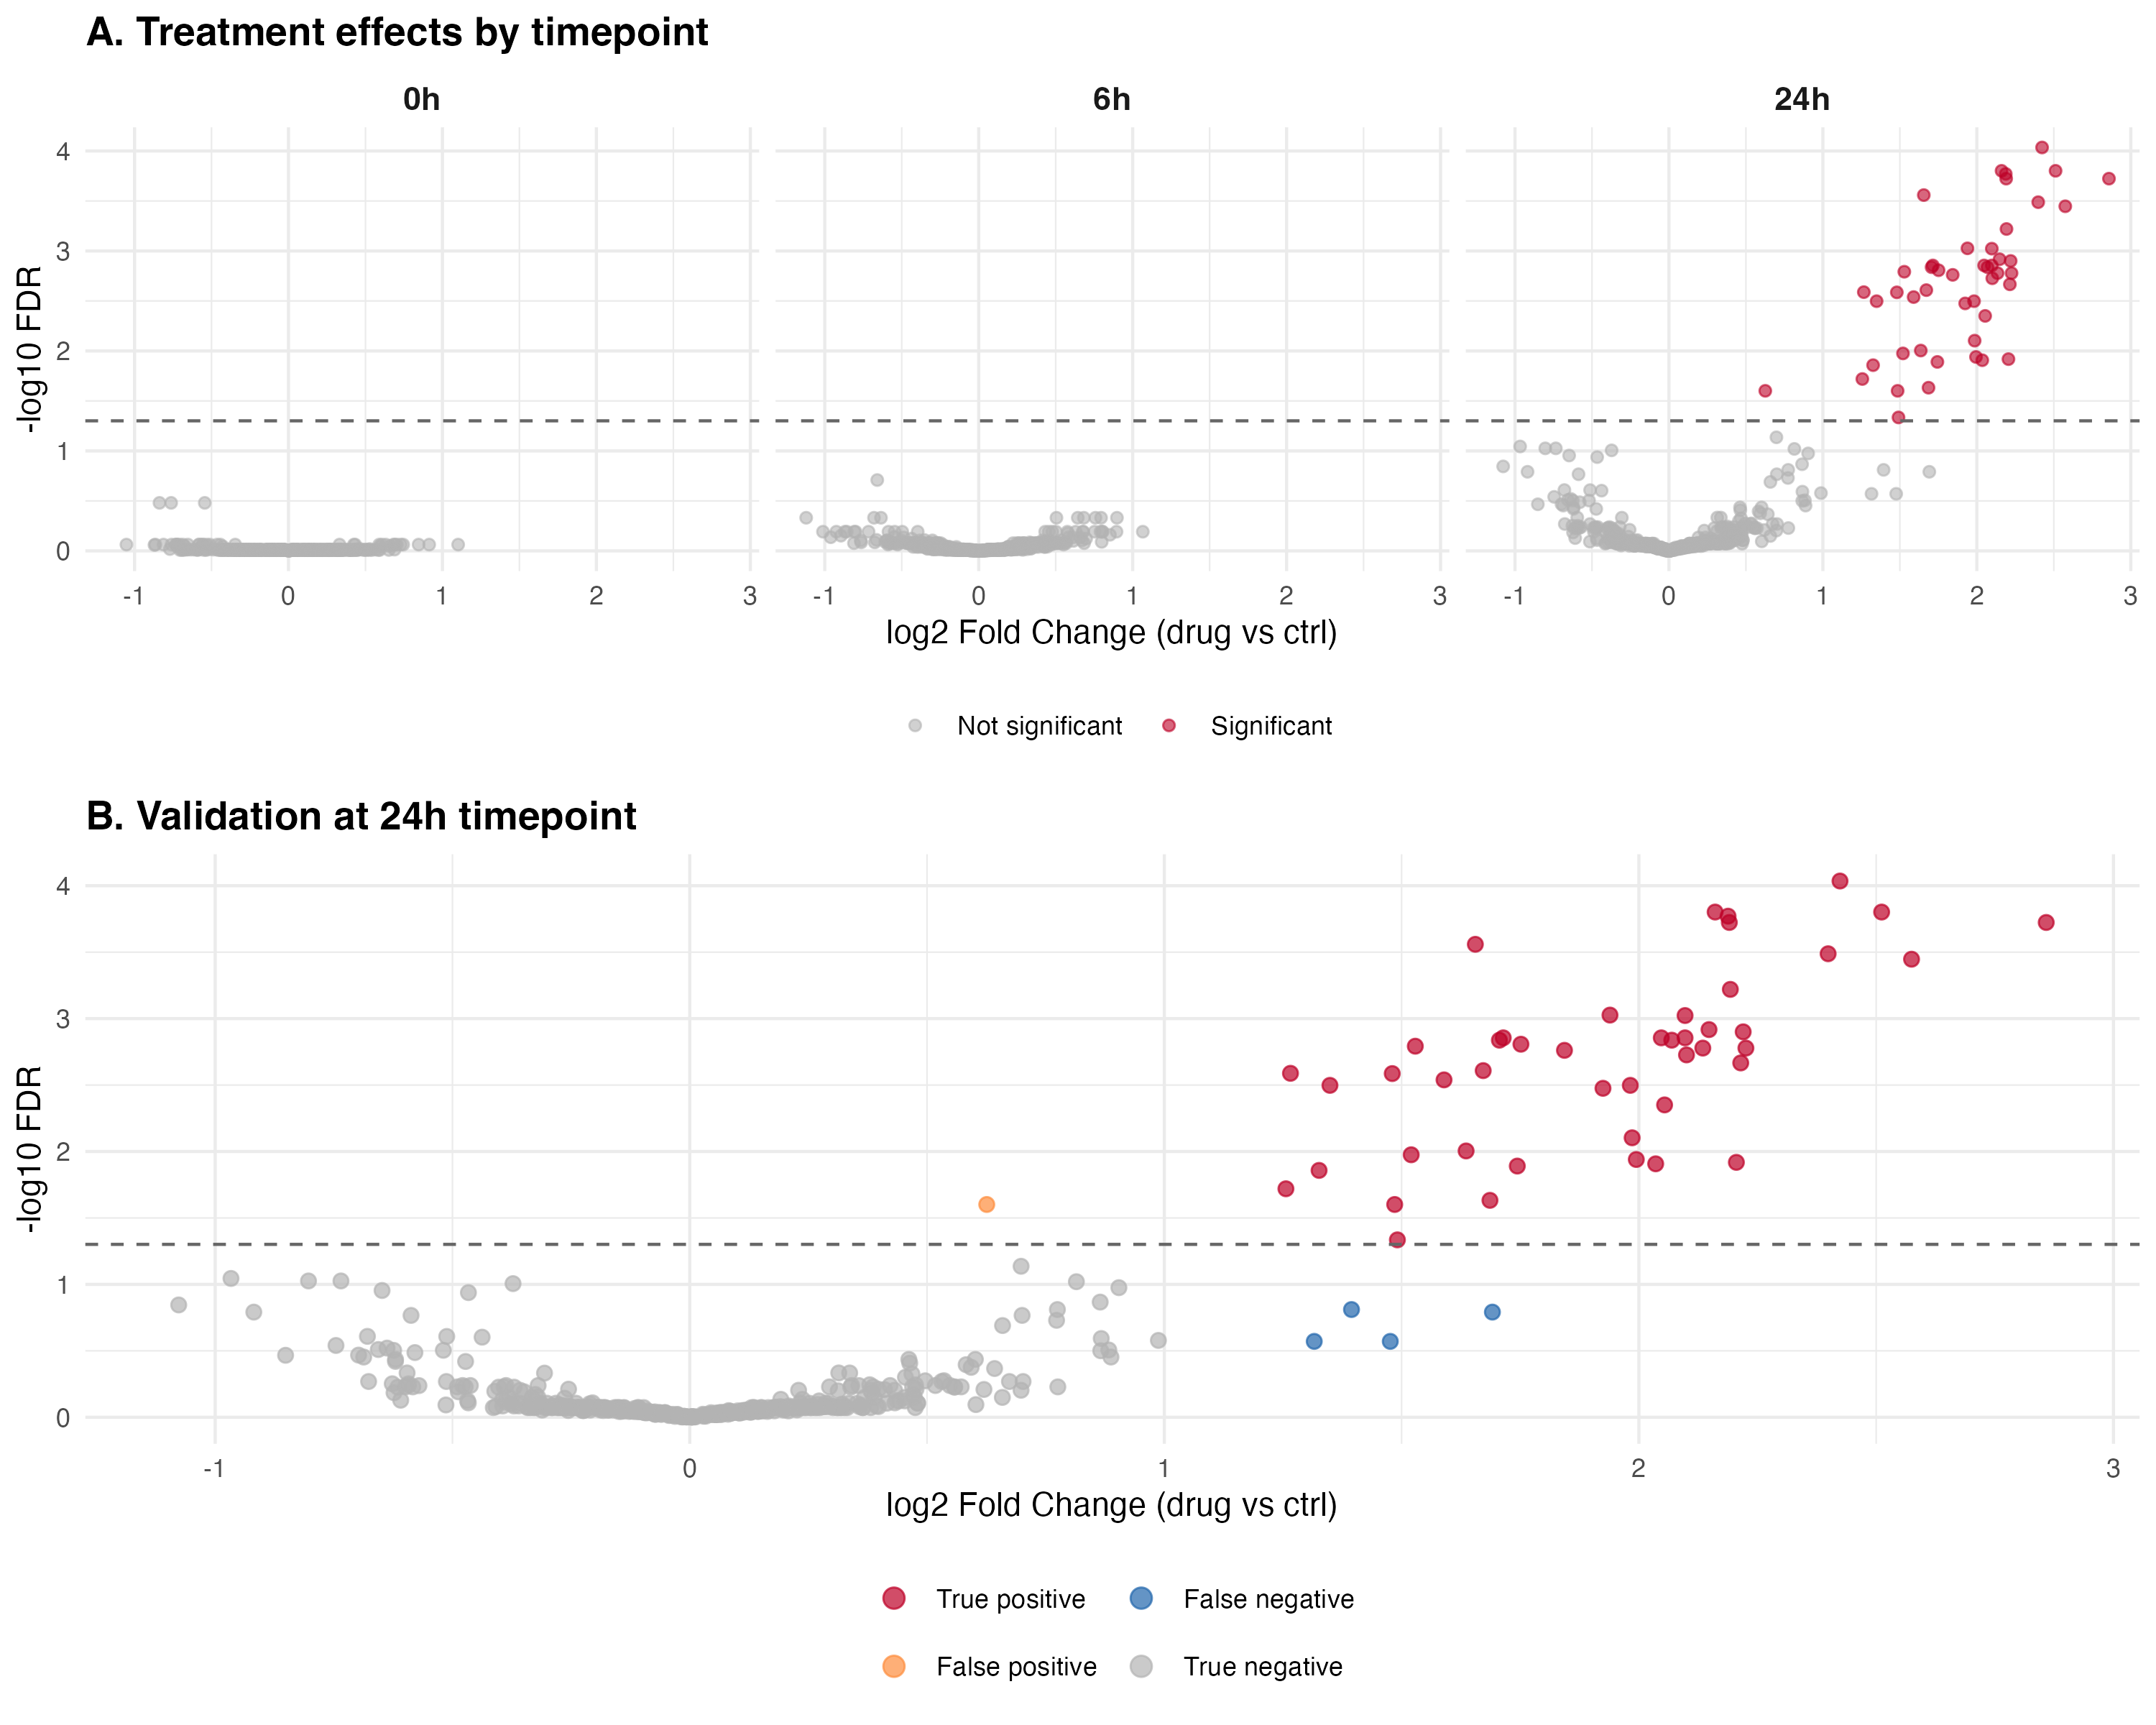
\includegraphics[keepaspectratio]{figure_1.pdf}}
\caption{Figure 1. Stratified analysis captures timepoint-specific
effects. (A) Volcano plots of treatment effects at each timepoint show
significant differences only at 24 hours, where true effects were
simulated. Dashed line indicates FDR = 0.05. (B) The 24-hour volcano
plot annotated with ground truth: red points are true positives (46/50
detected), blue points are false negatives (4/50 missed), and grey
points are true negatives. One false positive was detected.}
\end{figure}

\section{Discussion}\label{discussion}

pepdiff simplifies stratified factorial analysis for proteomics
experiments by automating contrast specification. The package uses
established statistical methods---Gamma GLMs with emmeans
contrasts---through an interface that does not require users to manually
code design matrices. Results are comparable to careful manual analysis;
the primary benefit is accessibility rather than statistical novelty.

Our simulations illustrate the value of matching analysis to
experimental design. In the factorial example, stratified analysis
captured timepoint-specific effects, while pooled analysis did not
detect significant differences because effects were present at only one
timepoint. The conventional workflow achieved similar sensitivity to
pepdiff when applied to the correct timepoint, though this required
prior knowledge of when to look. In practice, stratified analysis
examines all timepoints simultaneously without requiring such knowledge.

Several limitations apply. pepdiff models each peptide independently
without borrowing information across peptides, unlike hierarchical
approaches in tools such as limma. The package assumes cross-sectional
factorial designs with independent biological replicates; longitudinal
studies with repeated measures require different methods. The Gamma GLM
assumes positive, continuous abundance values; while spectral counts are
technically discrete, they are commonly treated as continuous in the
literature and the Gamma model performs adequately for these data.
Binary presence/absence data require alternative approaches.

pepdiff, together with peppwR for power analysis, provides a workflow
for factorial phosphoproteomics experiments from experimental design
through differential abundance analysis.

\section{Funding}\label{funding}

This work was supported by the Gatsby Charitable Foundation.

\section*{References}\label{references}
\addcontentsline{toc}{section}{References}

\protect\phantomsection\label{refs}
\begin{CSLReferences}{1}{0}
\bibitem[\citeproctext]{ref-benjamini1995fdr}
Benjamini, Yoav, and Yosef Hochberg. 1995. {``Controlling the False
Discovery Rate: A Practical and Powerful Approach to Multiple
Testing.''} \emph{Journal of the Royal Statistical Society: Series B
(Methodological)} 57 (1): 289--300.
\url{https://doi.org/10.1111/j.2517-6161.1995.tb02031.x}.

\bibitem[\citeproctext]{ref-breitling2004rankprod}
Breitling, Rainer, Patricia Armengaud, Anna Amtmann, and Pawel Herzyk.
2004. {``Rank Products: A Simple, yet Powerful, New Method to Detect
Differentially Regulated Genes in Replicated Microarray Experiments.''}
\emph{FEBS Letters} 573 (1-3): 83--92.
\url{https://doi.org/10.1016/j.febslet.2004.07.055}.

\bibitem[\citeproctext]{ref-choi2014msstats}
Choi, Meena, Ching-Yun Chang, Timothy Clough, Daniel Brouber, Trevor
Killeen, Brendan MacLean, and Olga Vitek. 2014. {``MSstats: An r Package
for Statistical Analysis of Quantitative Mass Spectrometry-Based
Proteomic Experiments.''} \emph{Bioinformatics} 30 (17): 2524--26.
\url{https://doi.org/10.1093/bioinformatics/btu305}.

\bibitem[\citeproctext]{ref-efron1993bootstrap}
Efron, Bradley, and Robert J Tibshirani. 1993. \emph{An Introduction to
the Bootstrap}. New York: Chapman; Hall/CRC.

\bibitem[\citeproctext]{ref-humphrey2015phosphoproteomics}
Humphrey, Sean J, S Babak Azimifar, and Matthias Mann. 2015.
{``High-Throughput Phosphoproteomics Reveals in Vivo Insulin Signaling
Dynamics.''} \emph{Nature Biotechnology} 33 (9): 990--95.
\url{https://doi.org/10.1038/nbt.3327}.

\bibitem[\citeproctext]{ref-lazar2016mnar}
Lazar, Cosmin, Laurent Gatto, Myriam Ferro, Christophe Bruley, and
Thomas Burger. 2016. {``Accounting for the Multiple Natures of Missing
Values in Label-Free Quantitative Proteomics Data Sets to Compare
Imputation Strategies.''} \emph{Journal of Proteome Research} 15 (4):
1116--25. \url{https://doi.org/10.1021/acs.jproteome.5b00981}.

\bibitem[\citeproctext]{ref-lenth2022emmeans}
Lenth, Russell V. 2022. {``Emmeans: Estimated Marginal Means, Aka
Least-Squares Means.''} \emph{R Package Version 1.8.0}.
\url{https://CRAN.R-project.org/package=emmeans}.

\bibitem[\citeproctext]{ref-maclean2026peppwr}
MacLean, Dan. 2026. {``peppwR: Simulation-Based Power Analysis for
Phosphoproteomics Experiments.''} \emph{Bioinformatics}.
\url{https://github.com/TeamMacLean/peppwR}.

\bibitem[\citeproctext]{ref-mccullagh1989glm}
McCullagh, Peter, and John A Nelder. 1989. \emph{Generalized Linear
Models}. 2nd ed. London: Chapman; Hall/CRC.

\bibitem[\citeproctext]{ref-olsen2006phosphoproteomics}
Olsen, Jesper V, Blagoy Blagoev, Florian Gnad, Boris Macek, Chanchal
Kumar, Peter Mortensen, and Matthias Mann. 2006. {``Global, in Vivo, and
Site-Specific Phosphorylation Dynamics in Signaling Networks.''}
\emph{Cell} 127 (3): 635--48.
\url{https://doi.org/10.1016/j.cell.2006.09.026}.

\bibitem[\citeproctext]{ref-ritchie2015limma}
Ritchie, Matthew E, Belinda Phipson, DI Wu, Yifang Hu, Charity W Law,
Wei Shi, and Gordon K Smyth. 2015. {``Limma Powers Differential
Expression Analyses for RNA-Sequencing and Microarray Studies.''}
\emph{Nucleic Acids Research} 43 (7): e47--47.
\url{https://doi.org/10.1093/nar/gkv007}.

\bibitem[\citeproctext]{ref-rouder2009bayest}
Rouder, Jeffrey N, Paul L Speckman, Dongchu Sun, Richard D Morey, and
Geoffrey Iverson. 2009. {``Bayesian t Tests for Accepting and Rejecting
the Null Hypothesis.''} \emph{Psychonomic Bulletin \& Review} 16 (2):
225--37. \url{https://doi.org/10.3758/PBR.16.2.225}.

\bibitem[\citeproctext]{ref-tyanova2016perseus}
Tyanova, Stefka, Tikira Temu, Pavel Sinitcyn, Arthur Carlson, Marco Y
Hein, Tamar Geiger, Matthias Mann, and Jürgen Cox. 2016. {``The Perseus
Computational Platform for Comprehensive Analysis of (Prote)omics
Data.''} \emph{Nature Methods} 13 (9): 731--40.
\url{https://doi.org/10.1038/nmeth.3901}.

\bibitem[\citeproctext]{ref-webb2015mnar}
Webb-Robertson, Bobbie-Jo M, Holli K Wiber, Melissa M Matzke, Joseph
Samuel, Margret Matthew, Marina A Gritsenko, Katrina M Waters, and Karin
D Rodland. 2015. {``Review, Evaluation, and Discussion of the Challenges
of Missing Value Imputation for Mass Spectrometry-Based Label-Free
Global Proteomics.''} \emph{Journal of Proteome Research} 14 (5):
1993--2001. \url{https://doi.org/10.1021/pr501138h}.

\bibitem[\citeproctext]{ref-wilcoxon1945}
Wilcoxon, Frank. 1945. {``Individual Comparisons by Ranking Methods.''}
\emph{Biometrics Bulletin} 1 (6): 80--83.
\url{https://doi.org/10.2307/3001968}.

\bibitem[\citeproctext]{ref-wobbrock2011art}
Wobbrock, Jacob O, Leah Findlater, Darren Gergle, and James J Higgins.
2011. {``The Aligned Rank Transform for Nonparametric Factorial Analyses
Using Only ANOVA Procedures.''} \emph{Proceedings of the SIGCHI
Conference on Human Factors in Computing Systems}, 143--46.
\url{https://doi.org/10.1145/1978942.1978963}.

\end{CSLReferences}

\end{document}
